\documentclass{beamer}

\usepackage{beamerthemeCambridgeUS}
\usepackage{textpos}
\usepackage{ragged2e}
\usepackage{ulem}
\graphicspath{{G:/My Drive/FIGURAS/}}

\title[Geoforma: Componente Interno]{GEOMORFOLOGÍA}
\author[Edier Aristizabal]{Edier V. Aristizábal G.}
\institute{evaristizabalg@unal.edu.co}
\date{\tiny{Versión:\today}}

\addtobeamertemplate{headline}{}{%
	\begin{textblock*}{2mm}(.9\textwidth,0cm)
	\hfill\includegraphics[height=1cm]{un}  
	\end{textblock*}}

\begin{document}
%%%%%%%%%%%%%%%%%%%%%%%%%%%%%%%%%%%%%%%%%%%%%%%%%%%%%%%%%%%%%%%%%%%%%%%%%
\begin{frame}
\titlepage
\centering
   	\includegraphics[width=4cm]{unal} 
\end{frame}
%%%%%%%%%%%%%%%%%%%%%%%%%%%%%%%%%%%%%%%%%%%%%%%%%%%%%%%%%%%%%%%%%%%%%%%%%
\begin{frame}
\frametitle{Morfocronología}
\centering
\includegraphics[scale=0.5]{morfocronologia}
\end{frame}
%%%%%%%%%%%%%%%%%%%%%%%%%%%%%%%%%%%%%%%%%%%%%%%%%%%%%%%%%%%%%%%%%%%%%%%%%%%
\begin{frame}
\frametitle{Técnicas de datación en geomorfología}
\centering
\includegraphics[scale=0.48]{columnacronologia}
\end{frame}
%%%%%%%%%%%%%%%%%%%%%%%%%%%%%%%%%%%%%%%%%%%%%%%%%%%%%%%%%%%%%%%%%%%%%%%%%%%
\begin{frame}
\frametitle{Técnicas de datación en geomorfología}
\centering
\includegraphics[scale=0.45]{estratigrafia}
\end{frame}
%%%%%%%%%%%%%%%%%%%%%%%%%%%%%%%%%%%%%%%%%%%%%%%%%%%%%%%%%%%%%%%%%%%%%%%%%%%
\begin{frame}
\frametitle{Líquenes}
\centering
\includegraphics[scale=0.5]{liquenes}
\end{frame}
%%%%%%%%%%%%%%%%%%%%%%%%%%%%%%%%%%%%%%%%%%%%%%%%%%%%%%%%%%%%%%%%%%%%%%%%%%%
\begin{frame}
\frametitle{Líquenes}
\framesubtitle{Bloques de rocas lisos, Dr. Eduardo Parra}
\centering
\includegraphics[scale=0.47]{liquenes1}
\end{frame}
%%%%%%%%%%%%%%%%%%%%%%%%%%%%%%%%%%%%%%%%%%%%%%%%%%%%%%%%%%%%%%%%%%%%%%%%%%%
\begin{frame}
\frametitle{Clasificación de cicatrices}
\framesubtitle{Dr. Eduardo Parra}
\centering
\includegraphics[scale=0.47]{cicatrices}
\end{frame}
%%%%%%%%%%%%%%%%%%%%%%%%%%%%%%%%%%%%%%%%%%%%%%%%%%%%%%%%%%%%%%%%%%%%%%%%%%%
\begin{frame}
\frametitle{Criterios temporales}
\framesubtitle{Dr. Eduardo Parra}
\centering
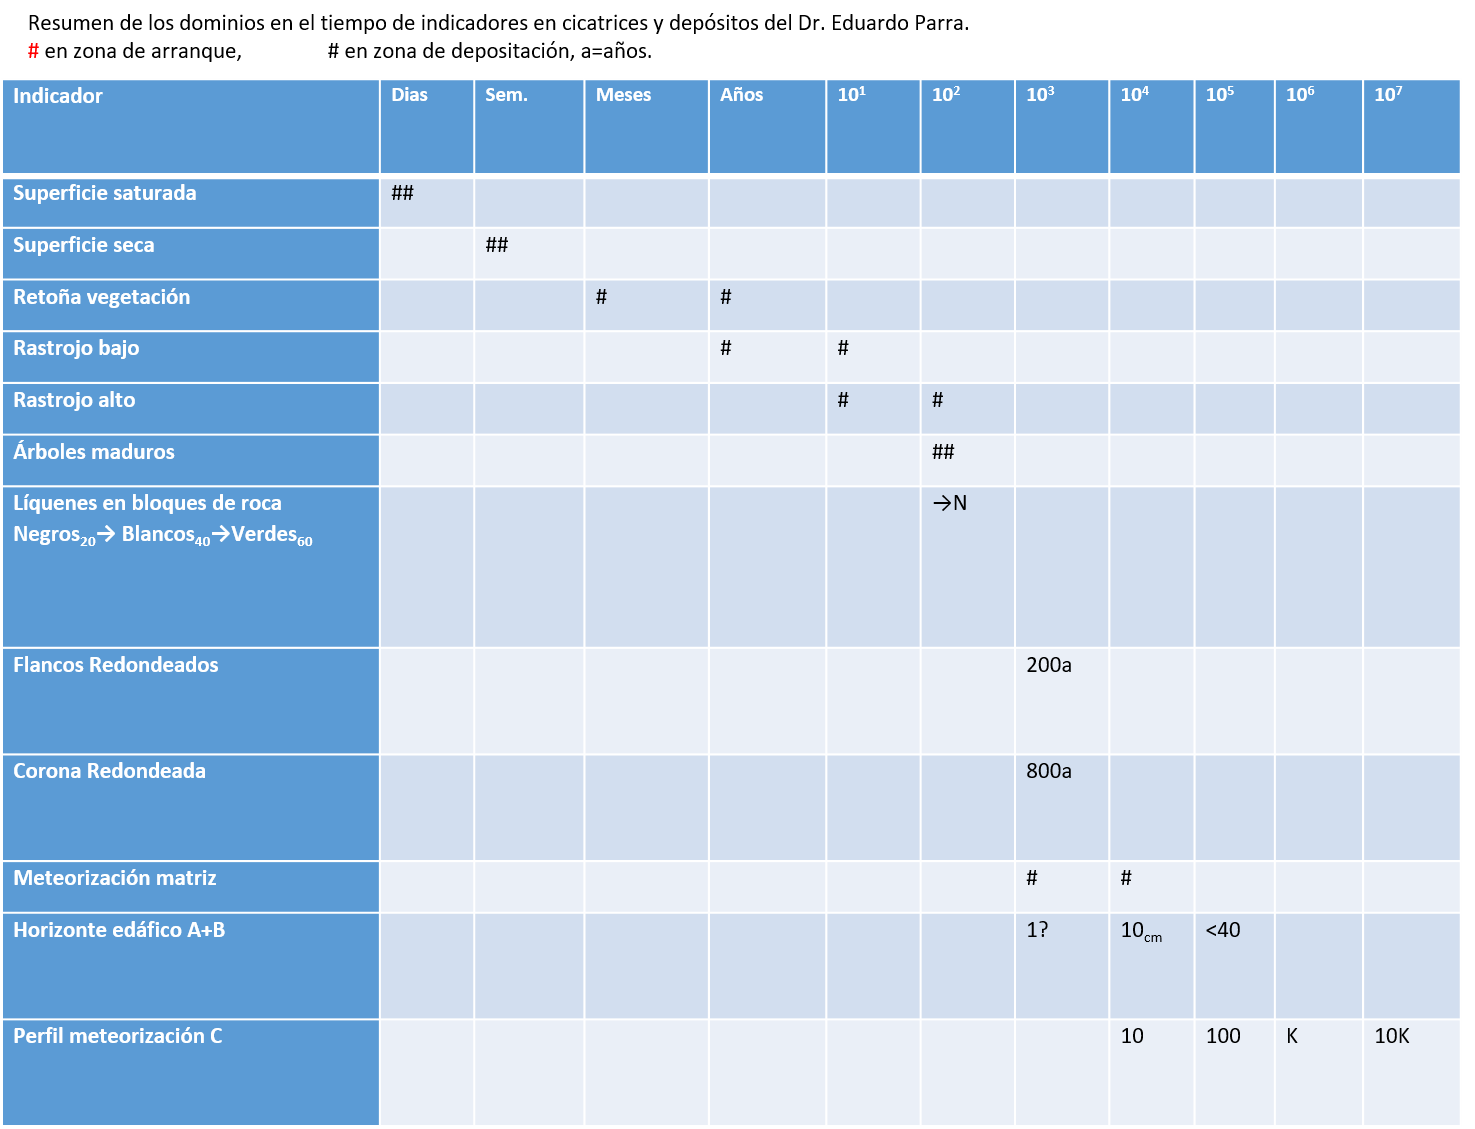
\includegraphics[scale=0.38]{tabla_parra}
\end{frame}
%%%%%%%%%%%%%%%%%%%%%%%%%%%%%%%%%%%%%%%%%%%%%%%%%%%%%%%%%%%%%%%%%%%%%%%%%%%
\begin{frame}
\frametitle{Ejemplo}
\centering
\includegraphics[scale=0.38]{piedragorda}
\end{frame}
%%%%%%%%%%%%%%%%%%%%%%%%%%%%%%%%%%%%%%%%%%%%%%%%%%%%%%%%%%%%%%%%%%%%%%%%%%%
\begin{frame}
\frametitle{Ejemplo}
\centering
\includegraphics[scale=0.38]{piedragorda1}
\end{frame}
%%%%%%%%%%%%%%%%%%%%%%%%%%%%%%%%%%%%%%%%%%%%%%%%%%%%%%%%%%%%%%%%%%%%%%%%%%%
\begin{frame}
\frametitle{Ejemplo: Antes}
\centering
\includegraphics[scale=0.45]{piedragorda_antes}
\end{frame}
%%%%%%%%%%%%%%%%%%%%%%%%%%%%%%%%%%%%%%%%%%%%%%%%%%%%%%%%%%%%%%%%%%%%%%%%%%%
\begin{frame}
\frametitle{Ejemplo: Durante}
\centering
\includegraphics[scale=0.45]{piedragorda_durante}
\end{frame}
%%%%%%%%%%%%%%%%%%%%%%%%%%%%%%%%%%%%%%%%%%%%%%%%%%%%%%%%%%%%%%%%%%%%%%%%%%%
\begin{frame}
\frametitle{Ejemplo: Despues}
\centering
\includegraphics[scale=0.45]{piedragorda_despues}
\end{frame}
%%%%%%%%%%%%%%%%%%%%%%%%%%%%%%%%%%%%%%%%%%%%%%%%%%%%%%%%%%%%%%%%%%%%%%%%%%%
\begin{frame}
\frametitle{Desintegración de elementos radioactivos}
\centering
\includegraphics[scale=0.45]{desintegracion}
\end{frame}
%%%%%%%%%%%%%%%%%%%%%%%%%%%%%%%%%%%%%%%%%%%%%%%%%%%%%%%%%%%%%%%%%%%%%%%%%%%
\begin{frame}
\frametitle{Desintegración de elementos radioactivos}
\centering
\includegraphics[scale=0.45]{desintegracion1}
\end{frame}
%%%%%%%%%%%%%%%%%%%%%%%%%%%%%%%%%%%%%%%%%%%%%%%%%%%%%%%%%%%%%%%%%%%%%%%%%%%
\begin{frame}
\frametitle{Métodos de datación absolutos}
\centering
\includegraphics[scale=0.45]{metodosdatacion}
\tiny{Fuente: Watchman \& Twidale (2002)}
\end{frame}
%%%%%%%%%%%%%%%%%%%%%%%%%%%%%%%%%%%%%%%%%%%%%%%%%%%%%%%%%%%%%%%%%%%%%%%%%%%
\begin{frame}
\frametitle{Isótopos cosmogénicos}
\small{Los isótopos cosmogénicos terrestres (TCN) producidos In Situ se producen por el resultado de la colisión de una partícula de alta energía (neutrones y muones) denominados rayos cósmicos contra un nucleido, el cual es roto en diversos fragmentos (espalación) que pueden ser: (i) radioactivos (14C, 10Be, 26Al, 36Cl), (ii) estables (3He, 21Ne). Para el caso de los estables la concentración del cosmogénico siempre se acumula en sucesivas exposiciones, el radioactivo no.}
\centering
\includegraphics[scale=0.45]{cosmogenicos}
\end{frame}
%%%%%%%%%%%%%%%%%%%%%%%%%%%%%%%%%%%%%%%%%%%%%%%%%%%%%%%%%%%%%%%%%%%%%%%%%%%
\begin{frame}
\frametitle{Isótopos cosmogénicos}
\centering
\includegraphics[scale=0.45]{cosmogenicos1}
\end{frame}
%%%%%%%%%%%%%%%%%%%%%%%%%%%%%%%%%%%%%%%%%%%%%%%%%%%%%%%%%%%%%%%%%%%%%%%%%%%
\begin{frame}
\frametitle{Isótopos cosmogénicos}
\centering
\includegraphics[scale=0.45]{cosmogenicos2}
\end{frame}
%%%%%%%%%%%%%%%%%%%%%%%%%%%%%%%%%%%%%%%%%%%%%%%%%%%%%%%%%%%%%%%%%%%%%%%%%%%
\begin{frame}
\frametitle{Isótopos cosmogénicos}
\framesubtitle{Carbono 14}
\centering
\includegraphics[scale=0.45]{c14}
\end{frame}
%%%%%%%%%%%%%%%%%%%%%%%%%%%%%%%%%%%%%%%%%%%%%%%%%%%%%%%%%%%%%%%%%%%%%%%%%%%
\begin{frame}
\frametitle{Isótopos cosmogénicos}
\framesubtitle{Tiempos de vida media}
\centering
\includegraphics[scale=0.45]{tiemposvida}
\end{frame}
%%%%%%%%%%%%%%%%%%%%%%%%%%%%%%%%%%%%%%%%%%%%%%%%%%%%%%%%%%%%%%%%%%%%%%%%%%%
\begin{frame}
\frametitle{Luminiscencia}
\centering
\includegraphics[scale=0.45]{luminiscencia}
\end{frame}
%%%%%%%%%%%%%%%%%%%%%%%%%%%%%%%%%%%%%%%%%%%%%%%%%%%%%%%%%%%%%%%%%%%%%%%%%%%
\begin{frame}
\frametitle{Luminiscencia}
\centering
\includegraphics[scale=0.45]{luminiscencia1}
\end{frame}
%%%%%%%%%%%%%%%%%%%%%%%%%%%%%%%%%%%%%%%%%%%%%%%%%%%%%%%%%%%%%%%%%%%%%%%%%%%
\begin{frame}
\frametitle{Dendrocronologia}
\centering
\includegraphics[scale=0.45]{dendrocronologia}
\end{frame}
%%%%%%%%%%%%%%%%%%%%%%%%%%%%%%%%%%%%%%%%%%%%%%%%%%%%%%%%%%%%%%%%%%%%%%%%%%%
\begin{frame}
\frametitle{Dendrocronologia}
\centering
\includegraphics[scale=0.45]{dendrocronologia1}
\end{frame}
%%%%%%%%%%%%%%%%%%%%%%%%%%%%%%%%%%%%%%%%%%%%%%%%%%%%%%%%%%%%%%%%%%%%%%%%%%%
\begin{frame}
\frametitle{Dendrogeomorfología}
\centering
\includegraphics[scale=0.45]{dendro}
\end{frame}
%%%%%%%%%%%%%%%%%%%%%%%%%%%%%%%%%%%%%%%%%%%%%%%%%%%%%%%%%%%%%%%%%%%%%%%%%%%
\end{document}